\section{Materials}
\addtocontents{toc}{\protect\setcounter{tocdepth}{2}}
As described in section \ref{subsubsec:method_classifier}, we train three classifiers on a dataset of social media texts containing offensive language. Using the trained models, Tweets in a test set can be classified. The models also serve to generate explanations for the classification result. The following section documents the implementation of the classifiers and the generation of explanations. Furthermore, we show the implementation of a graphical user interface (GUI) needed to evaluate the systems in a user study. The user study imposes another constraint: Participants can only be confronted with a limited amount of data points (Tweets). This section therefore also presents the selection of subsets to be shown in the user study.


\subsection{Dataset}

\subsubsection{Dataset Construction}
The original dataset was collected by Davidson et al. \cite{davidson2017automated} for their research on defining and differentiating hate speech from offensive language. They constructed a dataset with offensive Tweets and hate speech by conducting a keyword search on Twitter, using keywords registered in the hatebase dictionary\footnote{https://www.hatebase.org}. The timelines of Twitter users identified with the keyword search were scraped, resulting in a dataset of over 8 million Tweets. They selected 25 000 Tweets at random and had at least 3 annotators from Figure Eight\footnote{https://www.figure-eight.com} (formerly Crowd Flower) who labelled each Tweet as containing hate speech, offensive language, or neither. They reached an inter-annotator agreement of 0.92 \cite{davidson2017automated}. The dataset is publicly available on GitHub\footnote{https://github.com/t-davidson/hate-speech-and-offensive-language}.\newline
The biggest class in the dataset are the offensive language Tweets (77\%), while non-offensive Tweets represent 17\%, and hate speech 6\% of the dataset. \newline
For our research, we are interested in offensive and not offensive Tweets. The Tweets labelled as hate speech in this dataset have characteristics that offensive language does not necessarily have, i.e. is always pejorative, while offensive language can also be found in positive contexts (see \cite{davidson2017automated}). We therefore excluded Tweets labelled as hate speech for the further construction of our dataset. We produced a balanced dataset by selecting only Tweets with the maximum inter-annotator agreement from each of the two remaining classes, and randomly drew Tweets from the bigger class (offensive Tweets) until the size of the subset was equal to the size of the smaller class (non-offensive Tweets). Table \ref{tab:StatsDataset} presents statistical information about the resulting dataset.\newline
The dataset is split into a training set and a test set, with the test set containing 20\% of the data points. The training set is used to build the classifier models, while the Tweets of the test set are used to evaluate the classifiers and to generate the data points for the user study.
\begin{table}[!ht]
	\centering
	\begin{tabular}{lll}
		\textbf{} & \textbf{Not Offensive Class} & \textbf{Offensive Class} \\ \midrule
		Size (absolute) & 4,162 & 4,162 \\
		Size (relative) & 50.00\% & 50.00\% \\
		Total words & 58,288 & 61,504 \\
		Unique words & 6,437 & 9,855 \\
		\begin{tabular}[c]{@{}l@{}}Average words\\per Tweet\end{tabular} & 14.00 & 14.78 \\ \bottomrule         
	\end{tabular}
	\caption{Statistical characteristics of the constructed dataset}
	\label{tab:StatsDataset}
\end{table}


\subsubsection{Dataset Preprocessing}
To prepare the data to be used in a machine learning application, we adopt the following preprocessing steps (see section \ref{subsubsec:tweet_cleaning}) in chronological order:
\begin{enumerate}
	\item Conversion of all texts to lower cases
	\item Replacement of URLs by a dummy URL (``URL")
	\item Replacement of referenced user names and handles by a dummy handle (``USERNAME")
	\item This dataset encodes emojis in unicode decimal codes, e.g. ``\&\#128512;" for a grinning face. In order to keep the information contained in emojis, each emoji is replaced by its textual description (upper cased and without whitespaces to ensure unity for tokenizing)\footnote{https://www.quackit.com/character\_sets/emoji/}.
	\item Resolving contractions such as ``we're" or ``don't" by replacing contractions with their long version\footnote{https://en.wikipedia.org/wiki/Wikipedia:List\_of\_English\_contractions}.
	\item This dataset uses a few signifiers such as ``english translation" to mark a Tweet that has been translated to English, or ``rt" to mark a Retweet (i.e. a response to a previous Tweet). Since those information have been added retrospectively, we discard them here and delete the signifiers from the texts.
	\item Replacement of all characters that are non-alphabetic and not a hashtag by a whitespace
	\item Replacement of more than one subsequent whitespace by a single whitespace
	\item Tokenization on whitespaces
\end{enumerate}
After training the classifiers, the URL and username tokens are replaced by a more readable version (``http://website.com/website" and ``@username", respectively) to make it easier for participants of the user study to envision themselves in the scenario of a social media administrator reading real-world Tweets. Replacing the tokens by their original URLs and usernames would give the participants more information than the classifiers had; we therefore chose to use a dummy URL and username.\newline
Applying the preprocessing steps, the following Tweet is processed from its original form:
\medskip \hrule \medskip
\begin{verbatim}
	"@WBUR: A smuggler explains how he helped fighters along the \end{verbatim}\begin{verbatim}"Jihadi Highway": http://t.co/UX4anxeAwd"
\end{verbatim}
\medskip \hrule \medskip
into a cleaned version:
\medskip \hrule \medskip
\begin{verbatim}
@username a smuggler explains how he helped fighters along the \end{verbatim}\begin{verbatim}jihadi highway http://website.com/website
\end{verbatim}
\medskip \hrule \medskip



\subsection{Classifier}

\paragraph{Good System}
For the system with high accuracy (aiming 0.9 accuracy), we adopt the setup used by \cite{chen2018learning}. They achieve an accuracy of 0.9 in sentiment analysis on a movie review dataset (IMDB) with a convolutional neural network (CNN) and add their L2X algorithm to generate explanations for the CNN's decisions. The CNN consists of five layers, with an embeddings layer to transform sparse data into dense vectors, a convolution with subsequent pooling (max pooling with factor 2), a fully connected layer with 250 hidden dimensions, and an output layer with two nodes (see figure \ref{fig:impl_cnn}). Similar to \cite{chen2012detecting}, we use Categorical Cross-Entropy as loss function, and the Adam algorithm for optimisation. The L2X algorithm and the working example with a CNN on the IMDB dataset is publicly available on GitHub\footnote{https://github.com/Jianbo-Lab/L2X}. The CNN is implemented using the \textit{Keras}\footnote{https://keras.io} Python library with a TensorFlow\footnote{https://www.tensorflow.org} back end. With this setup, we achieve an accuracy of 0.9718 on our test set. 
\begin{figure} [!ht]
	\centering
	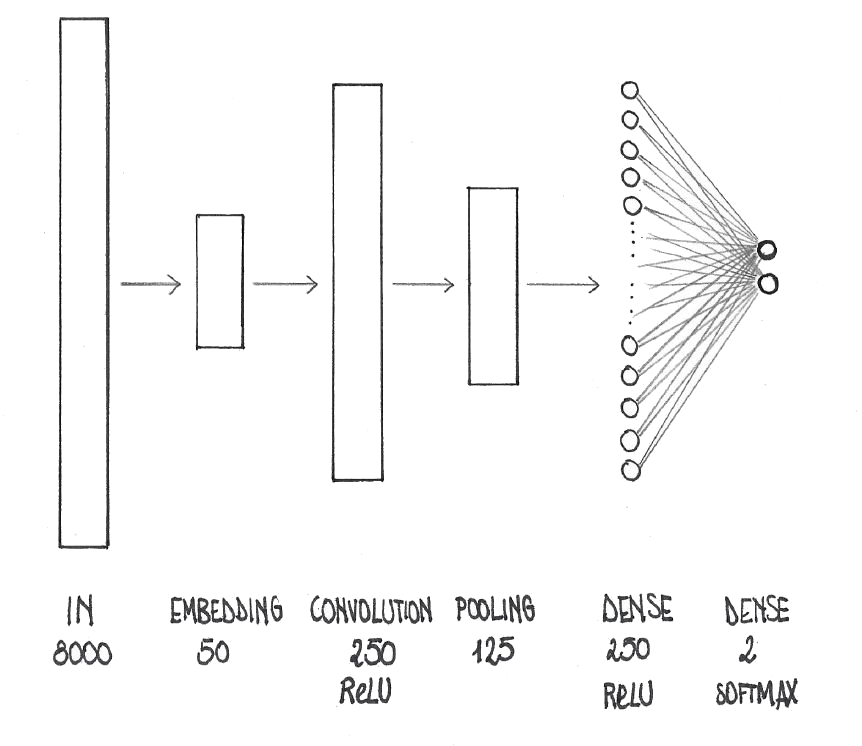
\includegraphics[width=0.7\textwidth]{img/impl_cnn.JPG}\\
	\caption{Architecture of the CNN with input vector and 5 layers, depicting layer goal, dimensionality, and activation function where applicable. Architecture adopted from \cite{chen2018learning}.}
	\label{fig:impl_cnn}
\end{figure}

\paragraph{Medium System}
In \cite{davidson2017automated}, logistic regression is used to identify offensive language and hate speech. They achieve an F1-score of 0.9 on their test set, with an L2 norm optimiser. We adopt the same setup, implementing a logistic regression classifier with the \textit{scikit-learn}\footnote{https://scikit-learn.org} Python library. We use the limited-memory BFGS algorithm for optimising and a fixed seed (random\_state=0) for shuffling the data. The dataset is encoded in a vector using the bag-of-words (BOW) method. The vocabulary of the training set is used for all further computations and out-of-vocabulary words are not considered. The accuracy on the training set of the logistic regression classifier is 0.9658. However, for the medium classifier, we aim for a system with an accuracy around 0.7\setcounter{footnote}{0}\renewcommand*{\thefootnote}{\fnsymbol{footnote}}\footnote{We also implemented a dictionary-based approach with characteristic words found by their tf-idf values, and a decision tree, with both methods reaching an accuracy of more than 0.9 - hence not applicable as a medium system.}\renewcommand*{\thefootnote}{\arabic{footnote}}\setcounter{footnote}{18}. Therefore, we reduce the resolution of all coefficients $c_i$ with $i \in \{0,I\}$, where $I$ is the number of coefficients (equal to the length of the vocabulary): 
\[c_i =
\begin{cases}
	-1 & \text{for   } c_i<0 \\
	+1 & \text{for   } c_i>0 \\
\end{cases}\]
The logistic regression classifier determines the probability estimate $p$ as:
\[
p=\frac{1}{1+e^{-(\alpha_0+\alpha_1x_1+\alpha_2x_2...+\alpha_ix_i)}}
\]
where $\alpha$ denotes the coefficients and $x$ the feature value. Since we encode the texts with BOW, all $x$ take a value of either $0$ (not present in Tweet) or $1$ (present in Tweet). The coefficients are binarised and either $-1$ (decisive for the non-offensive class) or $1$ (more influence towards the offensive class). As a result, the exponent of $e$ becomes \textit{positive} if the number of non-offensive words predominates in a text, and \textit{negative} if the Tweet contains more words decisive for the offensive class. With $e$ having a positive exponent, i.e. more words pivoting towards the non-offensive class, $p$ lies in the interval $]0.0,0.5[$. Contrarily, $p$ is in the interval $]0.5,1.0[$ for negative exponents (i.e. words decisive for the offensive class predominate the text). This approach is similar to the one used in \cite{klenner2018offensive}: After determining the class affiliation of the individual words in a text, they assign the class that has the most words in the text. The accuracy of the binarised logistic regression classifier on the test set is 0.7628.

\paragraph{Bad System}
The bad system is equal to the good classifier, but trained on a training set with inversed labels. The accuracy on the training set (with original labels) is 0.0282.



\subsection{Explanations} 
We chose the minimum explanation type that shows how input features relate to the classification result. In our use scenario, the input texts are Tweets with a maximum length of 140 characters. The average Tweet in the data set contains between 14 and 15 words (see table \ref{tab:StatsDataset}). We aim to select between $\frac{1}{3}$ and $\frac{1}{4}$ of the texts, which is around 4 words per Tweet. We assume that too few or too much words provide not enough or too much information to derive meaningful patterns. 


\paragraph{Good Explanations}
The \textit{medium classifier}, a logistic regression model, provides coefficients for each word in the training set vocabulary. We binarised the coefficients to reduce the classifier's accuracy to the desired level. For each Tweet, we therefore have a set of words working towards the non-offensive label, and another disjunct set of words adding to the offensive label. To generate an explanation with $k=4$ words, we draw at random $k$ words from the set of words working towards the predicted label. Theoretically, all words could be member of one set, and a truly truthful explanation would highlight all words. However, we choose to select only $k$ words to reach consistency with the explanations of the good classifier. An alternative would be the usage of the non-binarised coefficients. In that case, the user would have more detailed information than the classifier, which likewise results in a reduction of truthfulness. The medium system causes another issue: The encoding of texts with the BOW method omits the information about position within a sentence. If a word is selected that appears multiple times within a text, all instances contribute equally to the classification result and hence all instances have to be highlighted. The \textit{good classifier} using the \textit{L2X} algorithm analyses the global classification behaviour to generate local explanations. L2X tries to optimize the selection of features given the classification results - it learns ``a distribution over the subset of features given the input vector" \cite{chen2018learning} using an approximation of mutual information. For consistency with the medium classifier, all instances of a selected words in a Tweet are highlighted.

\paragraph{Bad Explanations}
As described in section \ref{subsubsec:method_explanations}, we generate nonsensical explanations by randomly drawing $k$ words from the Tweets. For consistency with the good explanations, all instances of a selected word are highlighted. The random word selection is done with the random number generator in the \textit{NumPy} Python library.

\paragraph{No Explanations}
In the case of no information at all, we select zero words per Tweet, hence no word is highlighted at all. Nevertheless, the user still receives the information about the classification result.



\subsection{Graphical User Interface}
For testing the effect of explanations of an automatic decision tool on users, we aim to create an authentic environment matching the use case scenario (see introduction to section \ref{sec:method}). The environment, in our case, is a software tool supporting the work of the ``social media administrator". The tool is a means to display the Tweets and the user interface to classify those Tweets. It also serves to show the classification result of the automatic decision system and its explanations.\newline
\begin{figure} [H]
	\centering
	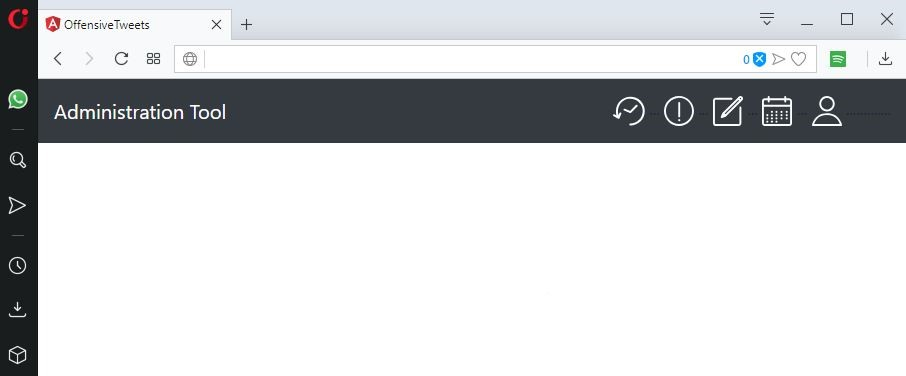
\includegraphics[width=0.8\textwidth]{img/administrationTool.JPG}
	\caption{Screenshot of the ``Administration Tool" to support the scenario of a social media administrator}
	\label{fig:admin_tool}
\end{figure}
\noindent The general layout of the software tool should remind the user of a modern web portal incorporating vital functions that are useful for a social media administrator (e.g. showing the social media profiles, showing the feed of the social media channels, reporting incidents, scheduling tasks, etc.). Furthermore, the user should believe that the system is capable of providing intelligent functionality, such as an automatic decision system. We therefore use the front-end web framework \textit{Bootstrap}\footnote{https://getbootstrap.com} to generate a modern and responsive web interface and include a menu bar with items for the various functionalities (see figure \ref{fig:admin_tool}). The interface design is minimalistic, as to not distract the user from the main task.\newline
The classifiers' decisions are visualised both with words and colours for an efficient usage. Texts classified as offensive have a red colouring, while a decision for the non-offensive class has a green colour scheme (see figure \ref{fig:admin_tool_offensive} and \ref{fig:admin_tool_not_offensive}). The colours are the extreme colours from the \textit{ColorBrewer}\footnote{http://colorbrewer2.org} ``RdYlGn" scale. The explanations are shown by highlighting words from the texts. We chose to display the Tweets in black font on a white background, while selected words are coloured according to the colour scheme.\newline
\begin{figure} [H]
	\centering
	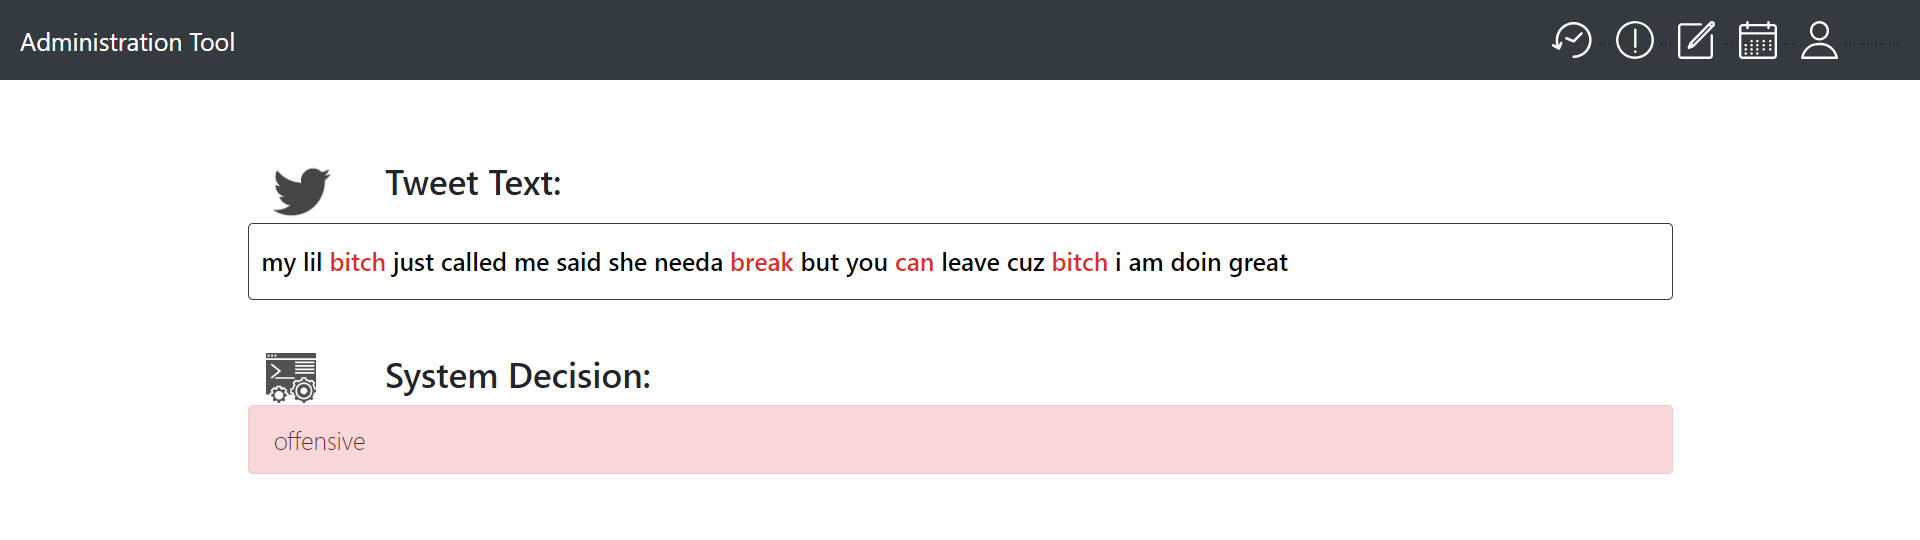
\includegraphics[width=0.8\textwidth]{img/pg_2_12.PNG}\\
	\caption{Screenshot of the ``Administration Tool" showing an offensive Tweet with explanation for its decision}
	\label{fig:admin_tool_offensive}
\end{figure}
\begin{figure} [H]
	\centering
	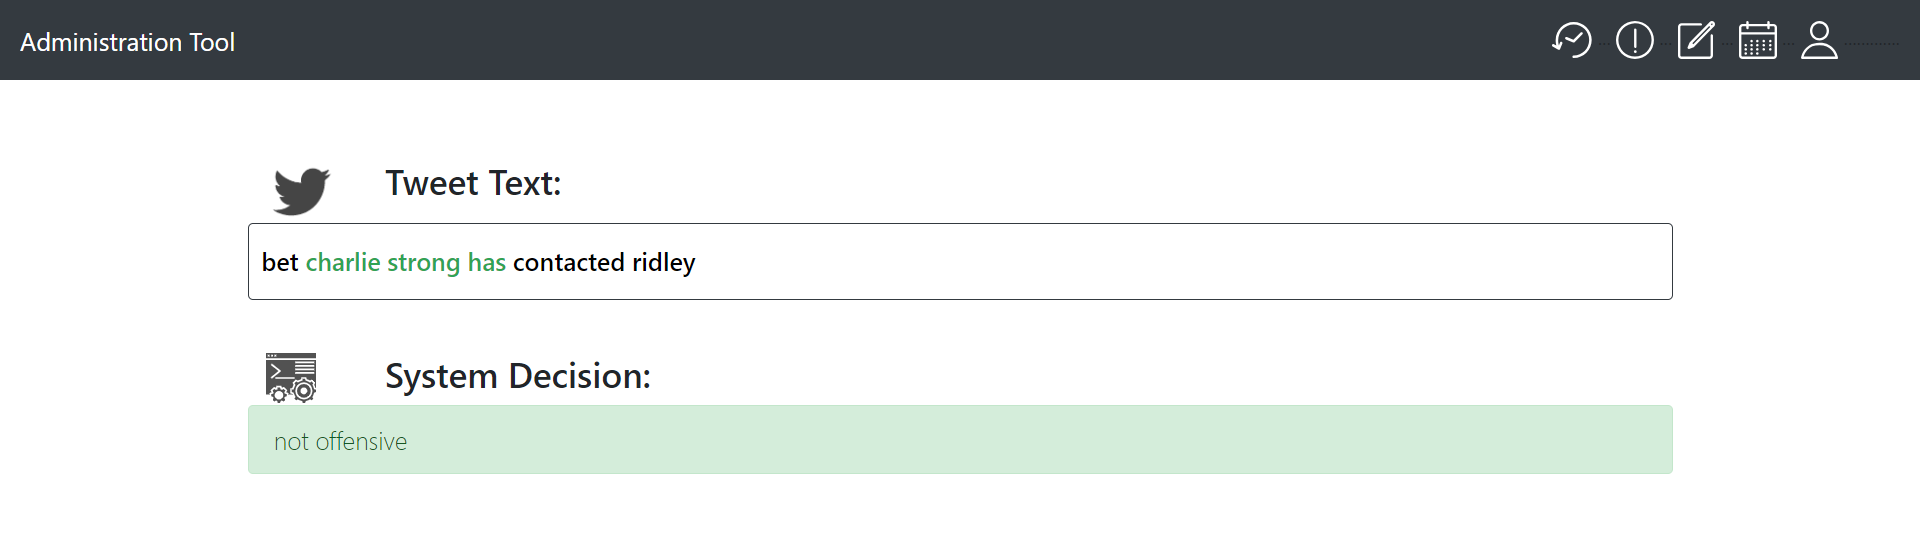
\includegraphics[width=0.8\textwidth]{img/pg_2_0.PNG}\\
	\caption{Screenshot of the ``Administration Tool" showing a non-offensive Tweet with explanation for its decision}
	\label{fig:admin_tool_not_offensive}
\end{figure}
\begin{figure}[H]
	\makebox[\textwidth][c]{
		\begin{minipage}[t]{0.25\textwidth}
			\centering
			
\includegraphics[width=\textwidth]{img/button_notoffensive.png}
		\end{minipage}%
		\hspace{5mm}
		\begin{minipage}[t]{0.25\textwidth}
			\centering
			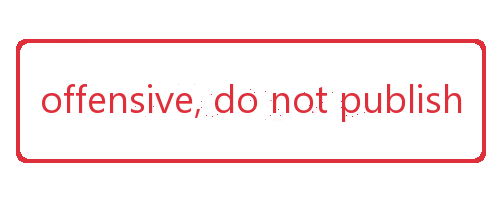
\includegraphics[width=\textwidth]{img/button_offensive.png}	
	\end{minipage}}
	\caption{Graphics of manual classification buttons matching the user interface}
	\label{fig:impl_buttons}
\end{figure}
\noindent Since the user study is run online and answers need to be registered within the survey tool, we convert the running system into static images by taking screenshots and incorporating the buttons used for user input directly in the survey tool as graphics (see figure \ref{fig:impl_buttons}). We automated the screenshot generation using \textit{Selenium}\footnote{https://www.seleniumhq.org}, a framework for automatic web application testing. The screenshots are taken with a size of 900x253 (in pixels, w x h).



\subsection{Subset Sampling}
For evaluating the different system-explanation conditions, users have to experience the system. However, it is not feasible to present them with the complete test set, since it has a size of 1665 Tweets. Consequently, a subset of Tweets needs to be drawn from the test set, with a size that a human observer can understand and process within the time frame of a user study.\newline
We furthermore aim to find 10 suitable subsets and assign participants randomly to one of the subsets, in order to reduce possible side effects from biases specific to single Tweets.\newline
There are several requirements for the subsamples, originating from the conflict of reducing the sample for a human observer, yet still yielding a good representation of the test set and classifier:\newline
\begin{itemize}
	\item A class balance of the true labels similar to the test set
	\item A balance of correctly to incorrectly classified data points similar to the classifier's performance on the complete test set
	\item No overlap of Tweets in between the 10 subsets and within a single subset
	\item A feature distribution close to the feature distribution in the complete test set
\end{itemize}
We set the subsample size to 15 Tweets, which is enough to show accuracies to the first decimal place, yet assumably not too much to process for an observer in a user study.\newline
To create a subset, 15 data points are randomly drawn from the test set. \newline
First, the class balance of the subset is calculated. The difference to the class balance of the whole test set needs to be smaller than 0.1.\newline
Additionally, for each classifier in the user study, the prediction accuracy on the subset is compared to the prediction accuracy on the complete test set. If, for all classifiers, the difference is smaller than 0.1, the next check is performed.\newline
To ensure the uniqueness of the subsets, the randomly drawn Tweets are compared with the content of previously found subsets. The subset is only accepted if none of the contained Tweets appear in any previously found subset.\newline
In the last step, the feature distribution of the subset is tested against the features of the complete test set using the \textit{Kullback-Leibler Divergence} (KLD) metric. As the focus is directed towards the explanations (i.e. the highlighted words within a Tweet), only the explanations are used to examine the feature distribution. First, the feature distribution of the complete test set is calculated by constructing a word vector with tuples of words and their respective word counts. The word counts are divided by the total amount of words in the set, such that the sum of regularised counts equals 1. Next, a copy of the word vector is used to count and regularise the word frequencies in the subset. The result are two comparable vectors, yet the vector of the subset is very likely to contain zero counts for words that appear in the complete set but were never selected as explanation in the subset. Since the KLD uses the logarithm, it is undefined for zero counts. We use Laplace smoothing with k=1 to handle zero counts. For each classifier, the KLD is calculated and summed to a total divergence score for the subset.\newline
We generate a quantity of 100 such subsets and order them by their KLD sum. The 10 subsets with the smallest score are chosen as the final set of subsets.\newline



{\color{blue}
\subsection{Explanation Evaluation}
\label{subsec:expleval}
experiments to validate whether the explanations we generate are actually ``good" explanations and those generated with the random method are actually ``bad" explanations.


\subsubsection{Evaluation 1: Accuracy on Reduced Texts}
For each system, take generated explanations of Tweets in the test set, reduce the text to the selected words, and feed the ``reduced Tweets" into the system. Hypothesis: If the words are very informative for the classifier, the accuracy would not change. The new accuracy should then be close to the old accuracy.\newline
\begin{figure}[H]
	\centering
	\begin{subfigure}[b]{0.4\textwidth}
		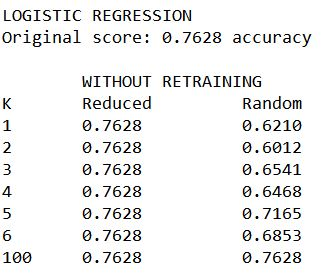
\includegraphics[width=\textwidth]{img/expleval1_logreg.JPG}
	\end{subfigure}
	\begin{subfigure}[b]{0.4\textwidth}
		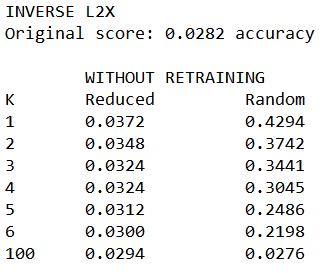
\includegraphics[width=\textwidth]{img/expleval1_invL2X.JPG}
	\end{subfigure}
	\caption{Results for evaluation of explanation experiment 1}
	\label{fig:results_expleval1}
\end{figure}
Problem: Tweets are very short, which is why the information density is high. Even when using only a single word randomly drawn from the text, the accuracy is 0.64, which is close to the medium classifier. It is therefore difficult to interpret the results for the medium classifier (0.76). Furthermore, we do not know if the Tweets have classified the same, or if only the accuracy is the same, but the mistakes were made on different Tweets. We therefore need to evaluate the ability to reproduce the very same classifications (evaluation 2).


\subsubsection{Evaluation 2: Ability to Reproduce Classifications}
For each system, divide the dataset in 5 chunks. Use each chunk once as test set and the remaining chunks as training set. This way, we get predictions and generated explanations for each data point in the dataset. Use the reduced version of the dataset with the predictions as truths to repeat the procedure of evaluation 1. Hypothesis: If the selected words are very informative for the classifier's prediction, the very same predictions can be reproduced with the reduced dataset. Since we take the predictions of the classifier on the non-reduced dataset as ``truth", the accuracy should be close to 1.0 .
\begin{figure}[H]
	\centering
	\begin{subfigure}[b]{0.4\textwidth}
		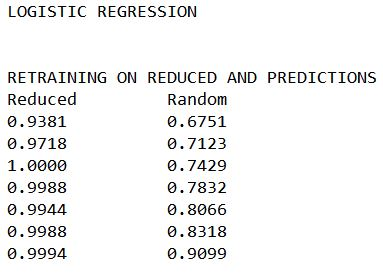
\includegraphics[width=\textwidth]{img/expleval2_logreg.JPG}
	\end{subfigure}
	\begin{subfigure}[b]{0.4\textwidth}
		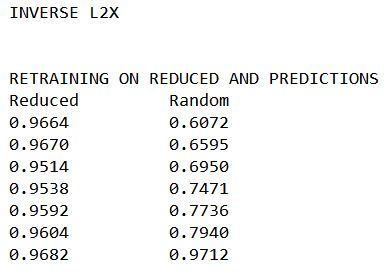
\includegraphics[width=\textwidth]{img/expleval2_invL2X.JPG}
	\end{subfigure}
	\caption{Results for evaluation of explanation experiment 2}
	\label{fig:results_expleval2}
\end{figure}



\subsection{Subset Evaluation}
same as previous section, but with the filtered subsets, basically. And on ``perfect" classifier. For k=4, because we use k=4 for final explanation generation.
}


\addtocontents{toc}{\protect\setcounter{tocdepth}{3}}